\chapter{Research}
\label{research}

\section{Architectures of Web Applications}

\section{Supporting Quality Requirements}

A key feature of any web application is the support of quality attributes, or non-functional requirements. There are many potential attributes that could be supported. What attributes are the key to the successful development of a web application? Software is evaluated by measuring quality attributes, though most software companies “have little motivation to improve the quality of their software” (Offutt 2002). This is not the case for web-based software which often relies not only on people going to their site, but “also returning to the site”. (Offutt 2002).  The key attributes for web applications identified were:

\begin {itemize}

\item	Reliability
\begin {itemize}
\item	Definition here
\end{itemize}

\item	Usability
\begin {itemize}
\item	Definition here
\end{itemize}

\item	Security
\begin {itemize}
\item	Definition here
\end{itemize}

\end{itemize}

Other quality attributes identified as important were

\begin {itemize}

\item	Availability
\begin {itemize}
\item	Definition here
\end{itemize}

\item	Scalability
\begin {itemize}
\item	Definition here
\end{itemize}

\item	Maintainability
\begin {itemize}
\item	Definition here
\end{itemize}

\item	Time to Market
\begin {itemize}
\item	Definition here
\end{itemize}

\end{itemize}

For the scope of this project, the focus shall be placed primarily on Usability and Security due to the nature of the website. Other non functional requirements, namely productivity, extensibility and maintainability, will be addressed in regards to the framework used to develop the web application.


\subsection{Measuring Usability}

\subsection{Measuring Extensibility}

\subsection{Measuring Security}

\subsection{Measuring Maintainability}

\subsection{Measuring Productivity }

\section{Architecture and Design Patterns}

\section{Technologies}

There are a number of components needs to build the architecture of a web application. The nature of these components is explored below, and their contribution to the creation of a web application is analysed.

\subsection{Web Application Framework}
The WAF chosen for this project is Spring MVC [Model View Controller]. Shan and Hua defined a WAF as “a defined support structure in which other software applications can be organized and developed”. (Shan and Hua 2006). Model-View-Controller is a software pattern that facilitates the use of a user interface. The Model manages the behaviour and data of the application. The View will manage the information obtained from the model and display it to the user. The Controller takes user input, such as key strokes, mouse movements or a touch display, and can interact and invoke functionality within the Model and/or View.

\begin{figure}[ht!]
\centering
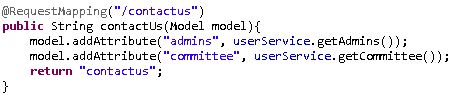
\includegraphics[width=90mm]{figs/fig3-4-1.jpg}
\caption{Contoller adding Model to View}
\label{overflow}
\end{figure}


\subsection{Application Server}

\subsection{Project Management Tool}

\subsection{Database Model}

\subsection{Source Control}

\subsection{Integrated Development Environment}

\subsection{Logging}

\subsection{Web Page Creation}

\section{Software Engineering}

\subsection{Requirements}

\subsection{Design}

\subsection{Testing}

\subsection{Software Quality}	